% exercise sheet with header on every page for math or close subjects
\documentclass[12pt]{article}
\usepackage[utf8]{inputenc} 
\usepackage{latexsym} 
\usepackage{multicol}
\usepackage{fancyhdr}
\usepackage{amsfonts} 
\usepackage{amsmath}
\usepackage{amssymb}
\usepackage{enumerate}
\usepackage{listings}
\usepackage{graphicx}
\usepackage{hyperref}

% Shortcuts for bb, frak and cal letters
\newcommand{\E}{\mathbb{E}}
\newcommand{\V}{\mathbb{V}}
\renewcommand{\P}{\mathbb{P}}
\newcommand{\N}{\mathbb{N}}
\newcommand{\R}{\mathbb{R}}
\newcommand{\C}{\mathbb{C}}
\newcommand{\Z}{\mathbb{Z}}
\newcommand{\Pfrak}{\mathfrak{P}}
\newcommand{\Pfrac}{\mathfrak{P}}
\newcommand{\Bfrac}{\mathfrak{P}}
\newcommand{\Bfrak}{\mathfrak{B}}
\newcommand{\Fcal}{\mathcal{F}}
\newcommand{\Ycal}{\mathcal{Y}}
\newcommand{\Bcal}{\mathcal{B}}
\newcommand{\Acal}{\mathcal{A}}

% formating
\topmargin -1.5cm 
\textheight 24cm
\textwidth 16.0 cm 
\oddsidemargin -0.1cm

% Fancy Header on every Page
\pagestyle{fancy}
\lhead{\textbf{Pattern and Speech Recognition}}
\rhead{Daniel Schäfer (2549458)\\ Christian Bohnenberger (2548364) \\ Dominik Weber (2548553)}
\renewcommand{\headrulewidth}{1.2pt}

\setlength{\headheight}{45pt} 

\begin{document}
\pagenumbering{gobble}

% TODO set the number of the exercise sheet here!
\setcounter{section}{6}
\setcounter{subsection}{1}

\subsection{ }

\begin{enumerate}[a)]
    \item   
        This statement is wrong because: Regularization is an method that reduces the generalization error but \textbf{not} the training error. (Source: Chapter 6 Slide 2)
    \item
        % TODO
        Not sure!
\end{enumerate}

\subsection{}
Both dropout and (boosting and) bagging are different methods to avoid overfitting.
Dropout can be seen as an extreme form of bagging in which each model is trained on a single case and each parameter of the model is very strongly regularized by sharing it with the corresponding parameter in all the other models which makes it an inexpensive approximation to bagging.
Boosting tries to improve the learners by focusing on learners where the system is not performing well by identifying significant errors and increasing the weight of this data in the next 'bagging-bag' which hopefully produces a better result. So boosting is an addon to Bagging where in subsequent bags we choose those data instances that have been modeled poorly in the overall system before.

\subsection{}
\begin{enumerate}[a)]
	\item 
		After $\tau$ steps, the components of the weight vector parallel to the eigenvectors of H can be written as:\\
			$$w^\tau_j= \{1-(1- \epsilon*\lambda)^\tau)\}*w^*_j $$ \\
		With $\tau \rightarrow \infty $ we get $(1- \epsilon*\lambda)^\tau)=0$ since we know $(1- \epsilon*\lambda)^\tau)<1$ by definition. Since:
		   $$lim_{\tau \rightarrow \infty} (w^\tau_j= \{1-(1- \epsilon*\lambda)^\tau)\}*w^*_j) = w^\tau_j= \{1-0\}*w^*_j$$\\
		   and \\
		   $$(w^\tau_j= \{1-0\}*w^*_j)= (w^\tau_j= w^*_j)$$
		   and this holds for all j and $w^\tau= w^\tau_0 \dots w^\tau_j$ for the max j and therefore we get:\\
		   $$ w^\tau \rightarrow w^* $$
		    
		
\end{enumerate}

\subsection{}
\begin{enumerate}[a)]
	\item 
		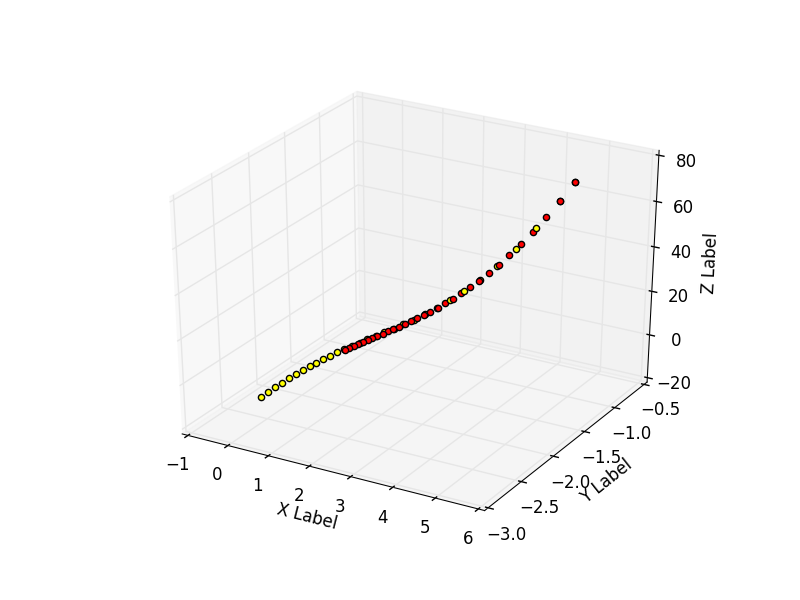
\includegraphics[scale=0.5]{figure_1.png}
		    
		
\end{enumerate}



\end{document}
